\documentclass[a4paper,11pt]{article}
\usepackage{amsmath}
\usepackage{amssymb}
\usepackage{fullpage}
\usepackage{rotating}
\usepackage{tikz} \usetikzlibrary{trees}

\newcommand{\AnyCond}[1]{\text{Any}(#1)}
\newcommand{\BoundedCond}[1]{\text{Bounded}(#1)}
\newcommand{\Constraint}[1]{\textsc{#1}}
\newcommand{\DepProps}{\textit{DepProps}}
\newcommand{\Distinct}{\Constraint{Distinct}}
\newcommand{\Element}{\Constraint{Element}}
\newcommand{\Failed}{\text{Failed}}
\newcommand{\FailedCond}[1]{\text{Failed}(#1)}
\newcommand{\FixedCond}[1]{\text{Fixed}(#1)}
\newcommand{\Fixpoint}{\text{AtFixpt}}
\newcommand{\NoneCond}[1]{\text{None}(#1)}
\newcommand{\Gecode}{\textit{Gecode}}
\newcommand{\GIST}{\textit{GIST}}
\newcommand{\Propagate}{\text{Propagate}}
\newcommand{\PropConds}[1]{\text{PropConds}(#1)}
\newcommand{\Sequence}[1]{\left[#1\right]}
\newcommand{\Set}[1]{\left\{#1\right\}}
\newcommand{\Subsumed}{\text{Subsumed}}
\newcommand{\Tuple}[1]{\left\langle#1\right\rangle}
\newcommand{\Unknown}{\text{Unknown}}

%Min commandon
\newcommand{\Tdots}{\, .\, .\,}

%\pagestyle{empty}

\renewcommand{\thesubsection}{\Alph{subsection}}
\renewcommand{\thesubsubsection}{\Alph{subsection}.\alph{subsubsection}}

\title{\textbf{Low-Level Parallel Programming \\
    Uppsala University -- Spring 2015 \\
    Report for Lab~1
    by Team~21  % replace t by your team number
  }
}

\author{Markus Palacios, Jonathan Sharyari} % replace by your name(s)

%\date{Month Day, Year}
\date{\today}


\begin{document}
\maketitle

\section{Questions}
\begin{description}
    \item[A] \textbf{What kind of parallelism is exposed in the identified method?}
 \hfill \\We have used task parallelism in the identified method. The vector containing the agents is been split up into the same number of processors of the running system, where each sub-vector is individually traversed by the deployed threads. As the same task is divided upon several threads, this is a type of data parallelism.
    \item[B] \textbf{How is the workload distributed across the threads?} \hfill \\The workload is distributed evenly across the threads. For pthreads, this means each thread gets equally many consecutive agents. Using OpenMP, the distribution is automatic, but using the standard settings, the same approach will be taken as with pthreads.
    \item[C] \textbf{Which number of thread gives you the best results? Why?} \hfill \\Our data suggests that the number of threads should generally be equal to the amount of processors in the system. In our case, the running system employs two virtual cores (SMT), which seems to benefit from the use of added threads, up to four, in the case of $OpenMP$ parallelisation (possibly due to hyperthreading). We believe the cause of $Pthreads'$ decline in performance is due to the greater overhead suffered. 
    \item[D] \textbf{Which version (OpenMP, Pthreads) gives you better results? Why?} \hfill \\As we can see in the figure \ref{figure1}, our graph shows that we get a much better result from using OpenMP as compared to Pthreads. As mentioned before this may be due to the larger overhead in Pthreads. When using Pthreads, it is up to the programmer to distribute the workload to the individual threads. We believe that the overheads of using pthreads, including creating and copying the in-data is too large. This could be overcome by moving the parallelism up in the code hierarchy; i.e., instead of craeting new threads each tick, threads may be created only once, continuously  maintaining a portion of the agents.
\end{description}

\section{How to run}
Without an argument specifying the type of parallelism, the serial version is used, whereas --pthreads and --openmp activates pthreads and openmp respectively (in case both are set, the last occurance will be dominating). The number of threads can in both cases be set by --np X. The value of X is ignored in the serial case.
\begin{description}
    \item[Serial] ./demo
    \item[OpenMP] ./demo --openmp
    \item[Pthreads] ./demo --pthreads --np 4
\end{description}
   
\subsection{Experiments}
Our experiments were run under Ubuntu Linux ~14.04 (64~bit) on an
Intel Core~i3~550 of 3.2~GHz with an 4~MB L2 cache and a 4~GB RAM.



\section*{Intellectual Property}
We certify that this report is solely produced by us, except where
explicitly stated otherwise and clearly referenced, and that we can
individually explain any part of it at the moment of submitting this
report.


\begin{figure}[h!]
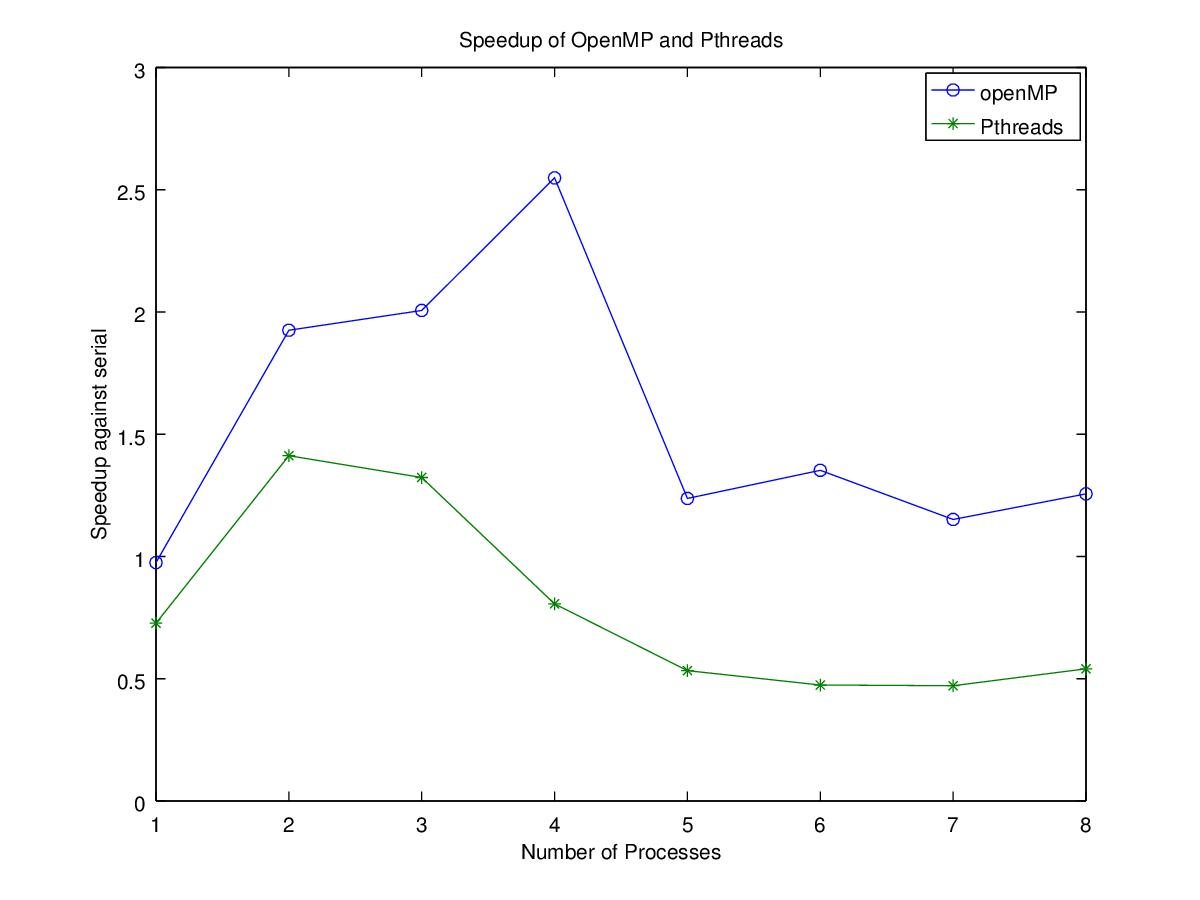
\includegraphics[width=\textwidth]{graph.jpg}
\caption{Graph showing the speedup of openmp and pthreads for 1 to 8 threads.}
\label{figure1}
\end{figure}



\end{document}
